\section{\oqasm: An Assembly Language for Quantum Oracles}
\label{sec:vqir}

We designed \oqasm to be able to express efficient quantum
oracles that can be easily tested and, if desired, proved
correct.
\oqasm operations leverage both the standard
computational basis and an alternative basis connected by the quantum
Fourier transform (QFT). 
\oqasm's type system tracks the bases of variables in
\oqasm programs, forbidding operations that would introduce
entanglement. \oqasm states are therefore efficiently
represented, so programs can be effectively tested and are simpler to
verify and analyze. In addition, \oqasm uses \emph{virtual qubits}
to support \emph{position shifting operations}, which support
arithmetic operations without introducing extra gates during
translation. All of these features are novel to quantum assembly
languages. 

This section presents \oqasm states and the language's syntax,
semantics, typing, and soundness results.  As a running example, we use the QFT
adder~\cite{qft-adder} shown in \Cref{fig:circuit-example}. The Coq
function \coqe{rz_adder} generates an \oqasm program that adds two
natural numbers \coqe{a} and \coqe{b}, each of length \coqe{n} qubits.

\begin{figure*}[t]
  \centering
  \begin{tabular}{c @{\quad} c}
  \begin{minipage}[b]{.55\textwidth}
  % 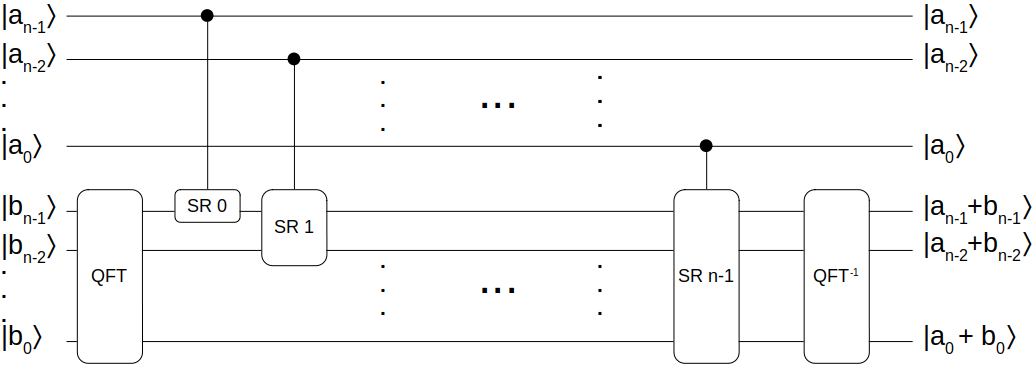
\includegraphics[width=1\textwidth]{qft-adder.png}
    \Small
    \Qcircuit @C=0.5em @R=0.75em {
      \lstick{\ket{a_{n-1}}} & \qw & \ctrl{5} & \qw & \qw & \qw & \qw & \qw & \qw & \qw & \rstick{\ket{a_{n-1}}} \\
      \lstick{\ket{a_{n-2}}} & \qw & \qw & \ctrl{4} & \qw & \qw & \qw & \qw & \qw & \qw & \rstick{\ket{a_{n-2}}}\\
      \lstick{\vdots} & & & & & & & & & & \rstick{\vdots} \\
      \lstick{} & & & & & & & & & & \\
      \lstick{\ket{a_0}} & \qw & \qw & \qw & \qw & \qw & \qw & \ctrl{1} & \qw & \qw & \rstick{\ket{a_0}} \\
      \lstick{\ket{b_{n-1}}} & \multigate{5}{\texttt{QFT}} & \gate{\texttt{SR 0}} & \multigate{3}{\texttt{SR 1}} & \qw & \qw & \qw & \multigate{5}{\texttt{SR (n-1)}} & \multigate{5}{\texttt{QFT}^{-1}} & \qw & \rstick{\ket{a_{n-1} + b_{n-1}}} \\
      \lstick{} & & & & & \dots & & & & \\
      \lstick{\ket{b_{n-2}}} & \ghost{\texttt{QFT}} & \qw  &  \ghost{\texttt{SR 1}} & \qw & \qw & \qw & \ghost{\texttt{SR (n-1)}} & \ghost{\texttt{QFT}^{-1}} & \qw & \rstick{\ket{a_{n-2} + b_{n-2}}} \\
      \lstick{\vdots} & & & & & & & & & & \rstick{\vdots} \\
      \lstick{} & & & & & & & & & & \\
      \lstick{\ket{b_0}} & \ghost{\texttt{QFT}} & \qw & \qw & \qw & \qw & \qw & \ghost{\texttt{SR (n-1)}} & \ghost{\texttt{QFT}^{-1}}  & \qw & \rstick{\ket{a_0 + b_0}} 
      }
  \subcaption{Quantum circuit}
  \end{minipage} &
  \begin{minipage}[b]{.35\textwidth}
  \begin{coq}
  Fixpoint rz_adder' (a b:var) (n:nat) 
    := match n with 
       | 0 => ID (a,0)
       | S m => CU (a,m) (SR m b); 
                rz_adder' a b m
       end.
  Definition rz_adder (a b:var) (n:nat) 
    := Rev a ; Rev b ; $\texttt{QFT}$ b ;
       rz_adder' a b n;
       $\texttt{QFT}^{-1}$ b; Rev b ; Rev a.
  \end{coq}
  \subcaption{\oqasm metaprogram (in Coq)}
  \end{minipage}
  \end{tabular}
  \vspace{-0.5em}
  \caption{Example \oqasm program: QFT-based adder}
  \label{fig:circuit-example}
  \end{figure*}

\subsection{\oqasm States} \label{sec:pqasm-states}

\begin{figure}[t]
  \small
  \[\hspace*{-0.5em}
\begin{array}{l>{$} p{1.2cm} <{$} c l}
      \text{Bit} & b & ::= & 0 \mid 1 \\
      \text{Natural number} & n & \in & \mathbb{N} \\
      \text{Real} & r & \in & \mathbb{R}\\
      \text{Phase} & \alpha(r) & ::= & e^{2\pi i r} \\
      \text{Basis} & \tau & ::= & \texttt{Nor} \mid \texttt{Phi}\;n \\
      \text{Unphased qubit} & \overline{q} & ::= & \ket{b} ~~\mid~~ \qket{r} \\
      \text{Qubit} & q & ::= &\alpha(r) \overline{q}\\
      \text{State (length $d$)} & \varphi & ::= & q_1 \otimes q_2 \otimes \cdots \otimes q_d
    \end{array}
  \]
  \caption{\oqasm state syntax}
  \label{fig:vqir-state}
\end{figure}

An \oqasm program state is represented according to the grammar in
\Cref{fig:vqir-state}. A state $\varphi$ of $d$ qubits is 
a length-$d$ tuple of qubit values $q$; the state models the tensor
product of those values. This means that the size of $\varphi$ is
$O(d)$ where $d$ is the number of qubits. A $d$-qubit state in a
language like \sqir is represented as a length $2^d$ vector of complex
numbers, which is $O(2^d)$ in the number of qubits.  Our linear state
representation is possible because applying any well-typed \oqasm
program on any well-formed \oqasm state never causes qubits to be
entangled.

A qubit value $q$ has one of two forms $\overline{q}$, scaled by a
global phase $\alpha(r)$. The two forms depend on the \emph{basis}
$\tau$ that the qubit is in---it could be either \texttt{Nor} or \texttt{Phi}. A \texttt{Nor} qubit has form
$\ket{b}$ (where $b \in \{ 0, 1 \}$), which is a
computational basis value. 
A \texttt{Phi} qubit has form $\qket{r} = \frac{1}{\sqrt{2}}(\ket{0}+\alpha(r)\ket{1})$, which is a value of the (A)QFT basis.
The number $n$ in \texttt{Phi}$\;n$ indicates the precision of the state $\varphi$.
As shown by~\citet{qft-adder}, arithmetic on the computational basis can sometimes be more efficiently carried out on the QFT basis, which leads to the use of quantum operations (like QFT) when implementing circuits with classical input/output behavior.
 
\subsection{\oqasm Syntax, Typing, and Semantics}\label{sec:oqasm-syn}

\liyi{add RZ gate back}

\begin{figure}[t]
\begin{minipage}[t]{0.5\textwidth}
{\small \centering

  $ \hspace*{-0.8em}
\begin{array}{llcl}
      \text{Position} & p & ::= & (x,n) \qquad   \text{Nat. Num}~n
                                  \qquad   \text{Variable}~x\\
      \text{Instruction} & \instr & ::= & \iskip{p} \mid \inot{p}
                                          \mid \irz[\lbrack -1 \rbrack]{n}{p} \mid \iseq{\instr}{\instr}\\
                & & \mid &  \isr[\lbrack -1 \rbrack]{n}{x} \mid \iqft[\lbrack -1 \rbrack]{n}{x} \mid \ictrl{p}{\instr}  \\
                      & & \mid & \ilshift{x} \mid \irshift{x} \mid \irev{x} 
    \end{array}
  $
}
  \caption{\oqasm syntax. For an operator \texttt{OP}, $\texttt{OP}^{\lbrack -1 \rbrack}$ indicates that the operator has a built-in inverse available.}
  \label{fig:vqir}
\end{minipage}
\hfill
\begin{minipage}[t]{0.45\textwidth}
\centering
\begin{tabular}{c@{$\quad=\quad$}c}
  \begin{minipage}{0.3\textwidth}
  \Small
%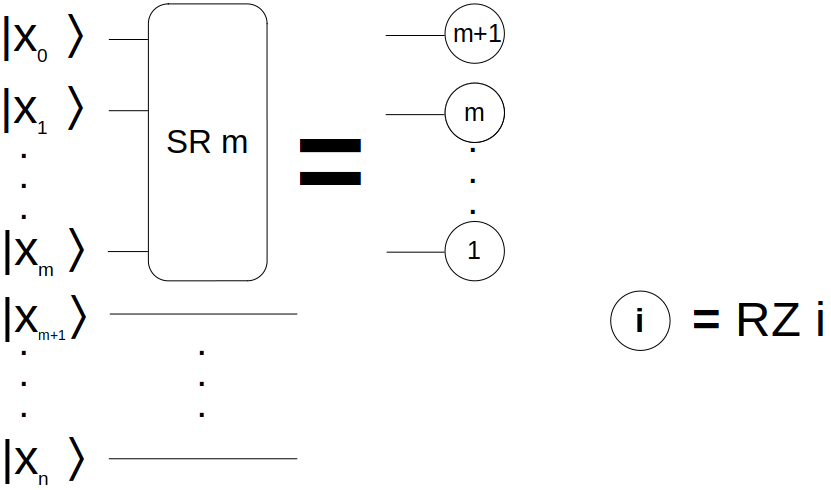
\includegraphics[width=0.3\textwidth]{sr-meaning.png}
  \Qcircuit @C=0.5em @R=0.5em {
    \lstick{} & \qw     & \multigate{4}{\texttt{SR m}} & \qw & \qw \\
    \lstick{} & \qw     & \ghost{\texttt{SR m}}           & \qw & \qw \\
    \lstick{} & \vdots & & \vdots & \\
    \lstick{} & & & & \\
    \lstick{} & \qw     & \ghost{\texttt{SR m}}           & \qw  & \qw
    }
  \end{minipage} & 
  \begin{minipage}{0.3\textwidth}
  \Small
  \Qcircuit @C=0.5em @R=0.5em {
    \lstick{} & \qw     & \gate{\texttt{RZ (m+1)}} & \qw & \qw \\
    \lstick{} & \qw     & \gate{\texttt{RZ m}}          & \qw & \qw \\
    \lstick{} & & \vdots & & \\
    \lstick{} & & & & \\
    \lstick{} & & & & \\
    \lstick{} & \qw     & \gate{\texttt{RZ 1}}           & \qw  & \qw
    }
  \end{minipage} 
\end{tabular}
\caption{\texttt{SR} unfolds to a series of \texttt{RZ} instructions}
\label{fig:sr-meaning}
\end{minipage}
\end{figure}

\Cref{fig:vqir} presents \oqasm's syntax. An \oqasm program consists of
a sequence of instructions $\instr$. Each instruction applies an
operator to either a variable $x$, which represents a group of qubits,
or a \emph{position} $p$, which identifies a particular offset into a variable $x$. 

The instructions in the first row correspond to simple single-qubit
quantum gates---$\iskip{p}$, $\inot{p}$, and $\irz[\lbrack -1 \rbrack]{n}{p}$
 ---and instruction sequencing.
The instructions in the next row apply to whole variables: $\iqft{n}{x}$
applies the AQFT to variable $x$ with $n$-bit precision and
$\iqft[-1]{n}{x}$ applies its inverse.
If $n$ is equal to the size of $x$, then the AQFT operation is exact.
$\isr[\lbrack -1 \rbrack]{n}{x}$
applies a series of \texttt{RZ} gates (\Cref{fig:sr-meaning}). 
Operation $\ictrl{p}{\instr}$
applies instruction $\instr$ \emph{controlled} on qubit position
$p$. All of the operations in this row---\texttt{SR}, \texttt{QFT}, and \texttt{CU}---will be translated to multiple \sqir
gates. Function \coqe{rz_adder} in \Cref{fig:circuit-example}(b) uses
many of these instructions; e.g., it uses \texttt{QFT} and \texttt{QFT}$^{-1}$ and applies
\texttt{CU} to the $m$th position of variable \texttt{a} to control
instruction \texttt{SR m b}.

In the last row of \Cref{fig:vqir}, instructions $\ilshift{x}$,
$\irshift{x}$, and $\irev{x}$ are \emph{position shifting operations}.
Assuming that $x$ has $d$ qubits and $x_k$ represents the $k$-th qubit
state in $x$, $\texttt{Lshift}\;x$ changes the $k$-th qubit state to
$x_{(k + 1)\% d}$, $\texttt{Rshift}\;x$ changes it to
$x_{(k + d - 1)\% d}$, and \texttt{Rev} changes it to $x_{d-1-k}$. In
our implementation, shifting is \emph{virtual} not physical. The \oqasm
translator maintains a logical map of variables/positions to concrete
qubits and ensures that shifting operations are no-ops, introducing no extra gates.

Other quantum operations could be added to \oqasm to
allow reasoning about a larger class of quantum programs, while still
guaranteeing a lack of entanglement. In \Cref{sec:extended-oqasm}, we
show how \oqasm can be extended to include the Hadamard gate
\texttt{H}, $z$-axis rotations \texttt{Rz}, and a new basis
\texttt{Had} to reason directly about implementations of QFT and AQFT\@.
However, this extension compromises the property of type reversibility
(\Cref{thm:reversibility}, \Cref{sec:metatheory}), and we have not found it necessary in
oracles we have developed.

\begin{figure}[t]
\begin{minipage}[t]{0.6\textwidth}
{\Small
  \begin{mathpar}
    \inferrule[X]{\Omegaty(x)=\texttt{Nor} \\ n < \Omegasz(x)}{\Sigma;\Omega \vdash \inot{(x,n)}\triangleright \Omega}
  
    \inferrule[RZ]{\Omegaty(x)=\texttt{Nor} \\ n < \Omegasz(x)}{\Sigma;\Omega \vdash \irz{q}{(x,n)} \triangleright \Omega}

    \inferrule[SR]{\Omegaty(x)=\tphi{n} \\ m < n}{\Sigma;\Omega \vdash \texttt{SR}\;m\;x\triangleright \Omega}   

    \inferrule[QFT]{\Omegaty(x)=\texttt{Nor}\\n \le \Omegasz(x)}{\Sigma; \Omega \vdash \iqft{n}{x}\triangleright \Omega[x\mapsto \tphi{n}]}    
     
    \inferrule[RQFT]{\Omegaty(x)=\tphi{n}\\n \le \Omegasz(x)}{\Sigma; \Omega \vdash \iqft[-1]{n}{x}\triangleright \Omega[x\mapsto \texttt{Nor}]}             
    
    \inferrule[CU]{\Omegaty(x)=\texttt{Nor} \\ \texttt{fresh}~(x,n)~\instr \\\\ \Sigma; \Omega\vdash \instr\triangleright \Omega \\ \texttt{neutral}(\instr)}{\Sigma; \Omega \vdash \texttt{CU}\;(x,n)\;\instr \triangleright \Omega} 
     
    \inferrule[LSH]{\Omegaty(x)=\texttt{Nor}}{\Sigma; \Omega \vdash \texttt{Lshift}\;x\triangleright \Omega}

     \inferrule[SEQ]{\Sigma; \Omega\vdash \instr_1\triangleright \Omega' \\ \Sigma; \Omega'\vdash \instr_2\triangleright \Omega''}{\Sigma; \Omega \vdash \instr_1\;;\;\instr_2\triangleright \Omega''} 
    
  \end{mathpar}
}
  \caption{Select \oqasm typing rules}
  \label{fig:exp-well-typed}
\end{minipage}
\hfill
\begin{minipage}[t]{0.35\textwidth}
{\footnotesize
\begin{center}\hspace*{-1em}
\begin{tikzpicture}[->,>=stealth',shorten >=1pt,auto,node distance=3.2cm,
                    semithick]
  \tikzstyle{every state}=[fill=black,draw=none,text=white]

  \node[state] (A)              {$\texttt{Nor}$};
  \node[state]         (C) [left of=A] {$\tphi{n}$};

  \path (A) edge [loop above]            node {$\Big\{\begin{array}{l}\texttt{ID},~\texttt{X},~\texttt{RZ}^{\lbrack -1 \rbrack},~\texttt{CU},\\
              \texttt{Rev},\texttt{Lshift},\texttt{Rshift}\end{array}\Big\}$} (A)
            edge   node [above] {\{$\texttt{QFT}\;n$\}} (C);
  \path (C) edge [loop above]            node {$\{\texttt{ID},~\texttt{SR}^{\lbrack -1 \rbrack}\}$} (C)
            edge  [bend right]             node {$\{\texttt{QFT}^{-1}\;n\}$} (A);
\end{tikzpicture}
\end{center}
}
\caption{Type rules' state machine}
\label{fig:state-machine}
\end{minipage}
\end{figure}

\myparagraph{Typing}
\label{sec:vqir-typing}

In \oqasm, typing is with respect to a \emph{type environment}
$\Omega$ and a predefined \emph{size
  environment} $\Sigma$, which map \oqasm
variables to their basis and size (number of qubits), respectively.
The typing judgment is written $\Sigma; \Omega\vdash \instr \triangleright \Omega'$ which
states that $\instr$ is well-typed under $\Omega$ and $\Sigma$, and
transforms the variables' bases to be as in $\Omega'$ ($\Sigma$ is unchanged). 
\liyi{good?}
$\Sigma$ is fixed because the number of qubits in an execution is always fixed.
It is generated in the high level language compiler, such as \sourcelang in \Cref{sec:qimp}.
The algorithm generates $\Sigma$ by taking an \sourcelang program and scanning through
all the variable initialization statements.
Select type rules are given in \Cref{fig:exp-well-typed}; 
the rules not shown (for \texttt{ID}, \texttt{Rshift}, \texttt{Rev}, \texttt{RZ}$^{-1}$, and \texttt{SR}$^{-1}$) are similar.

The type system enforces three invariants.  First, it enforces that
instructions are well-formed, meaning that gates are applied to valid
qubit positions (the second premise in \rulelab{X}) and that any control qubit is distinct from the
target(s) (the \texttt{fresh} premise in
\rulelab{CU}).  This latter property enforces the quantum
\emph{no-cloning rule}.
For example, we can apply the \texttt{CU} in \code{rz\_adder'} (\Cref{fig:circuit-example})
because position \code{a,m} is distinct from variable \code{b}.

Second, the type system enforces that instructions leave affected
qubits in a proper basis (thereby avoiding entanglement). The
rules implement the state machine shown in
\Cref{fig:state-machine}. For example, $\texttt{QFT}\;n$ transforms a variable from \texttt{Nor} to
$\tphi{n}$ (rule \rulelab{QFT}), while $\texttt{QFT}^{-1}\;n$
transforms it from $\tphi{n}$ back to \texttt{Nor} (rule
\rulelab{RQFT}). Position shifting operations 
are disallowed on variables $x$ in
the \texttt{Phi} basis because the qubits that make up $x$ are
internally related (see \Cref{def:well-formed}) and cannot be rearranged. Indeed, applying a
\texttt{Lshift} and then a $\texttt{QFT}^{-1}$ on $x$ in \texttt{Phi}
would entangle $x$'s qubits.

% \begin{figure}[t]
% {\footnotesize
% \begin{center}
% \begin{tikzpicture}[->,>=stealth',shorten >=1pt,auto,node distance=3.2cm,
%                     semithick]
%   \tikzstyle{every state}=[fill=white,draw=black,text=black]
% 
%   \node[initial,accepting,state] (A)              {$\texttt{OK}$};
%   \node[state]         (B) [right of=A] {$ $};
% 
%   \path (A) edge [loop above]            node {$b,\epsilon / \epsilon$} (A)
%             edge  [above] node {$a,\emptyset / a$} (B);
%   \path (B) edge [loop right]            node [right] {$\begin{array}{l}b,\epsilon / \epsilon\\
%                                                                 a,a' / a a'\\
%                                                                 a,\overline{a} / \epsilon\\
%                                                  \end{array}$} (B)
%             edge  [bend left]             node [above] {$\epsilon,\emptyset / \emptyset$} (A);
% \end{tikzpicture}
% \end{center}
% }
% {
% \footnotesize
% $
% \begin{array}{l}
% a,a'\in \{\ilshift{x},\irshift{x},\irev{x} \} \wedge a' \neq \overline{a}
% \\
% \overline{\ilshift{x}}=\irshift{x}
% \quad
% \overline{\irshift{x}}=\ilshift{x}
% \quad
% \overline{\irev{x}}=\irev{x}
% \\
% b\not\in\{\ilshift{x},\irshift{x},\irev{x}, \instr;\instr \}
% \\
% \emptyset=\text{ no element in stack}
% \end{array}
% $
% }
% 
% \caption{Pushdown automata for \texttt{neutral}}
% \label{fig:pushdown-neu}
% \end{figure}

Third, the type system enforces that the effect of position shifting
operations can be statically tracked. The \texttt{neutral} condition of
\rulelab{CU} requires that any shifting within $\instr$ is restored by the time it
completes. 
For example, $\sseq{\ictrl{p}{(\ilshift{x})}}{\inot{(x,0)}}$ is not well-typed, because knowing the final physical position of qubit $(x,0)$ would require statically knowing the value of $p$. 
On the other hand, the program $\sseq{\ictrl{c}{(\sseq{\ilshift{x}}{\sseq{\inot{(x,0)}}{\irshift{x}}})}}{\inot{(x,0)}}$ is well-typed 
because the effect of the \texttt{Lshift} is ``undone'' by an \texttt{Rshift} inside the body of the \texttt{CU}.

% \texttt{neutral}'s definition in \Cref{fig:pushdown-neu}
% views $\instr$ as a string concatenated
% by the sequence operation ($;$) and requires $\instr$ to be
% accepted according to a family of pushdown automatas $\{G\}_{x}$ for every $x$ presented in $\instr$. 
% A program $\instr$ is \texttt{neutral}, iff, $\instr$ as a string is
% accepted by all the automatas in $\{G\}_{x}$.

\myparagraph{Semantics}\label{sec:pqasm-dsem}

\begin{figure}[t]
{\footnotesize
\[
\begin{array}{lll}
\llbracket \iskip{p} \rrbracket\varphi &= \varphi\\[0.2em]

\llbracket \inot{(x, i)} \rrbracket\varphi &= \app{\uparrow\xsem(\downarrow\varphi(x,i))}{\varphi}{(x,i)}
& \texttt{where  }\xsem(\ket{0})=\ket{1} \qquad\, \xsem(\ket{1})=\ket{0}
\\[0.5em]

\llbracket \ictrl{(x,i)}{\instr} \rrbracket\varphi &=  \csem(\downarrow\varphi(x,i),\instr,\varphi)
&
\texttt{where  }
\csem({\ket{0}},{\instr},\varphi)=\varphi\quad\;\,
\csem({\ket{1}},{\instr},\varphi)=\llbracket \instr \rrbracket\varphi
\\[0.4em]

\llbracket \irz{m}{(x,i)} \rrbracket\varphi &= \app{\uparrow {\rsem}({m},\downarrow\varphi(x,i))}{\varphi}{(x,i)}
&\texttt{where  }{\rsem}(m,\ket{0})=\ket{0} \; \quad{\rsem}(m,\ket{1})=\alpha(\frac{1}{2^m})\ket{1}
\\[0.5em]

\llbracket \irz[-1]{m}{(x,i)} \rrbracket\varphi &= \app{\uparrow {\rrsem}({m},\downarrow\varphi(x,i))}{\varphi}{(x,i)}
 &\texttt{where  }{\rrsem}(m,\ket{0})=\ket{0}
\quad{\rrsem}(m,\ket{1})=\alpha(-\frac{1}{2^m})\ket{1}
\\[0.5em]

\llbracket \isr{m}{x} \rrbracket\varphi &
                                            \multicolumn{2}{l}{= \app{\uparrow \qket{r_i+\frac{1}{2^{m-i+1}}}}{\varphi}{\forall i \le m.\;(x,i)}
\qquad \texttt{when  }
\downarrow\varphi(x,i) = \qket{r_i}}\\[0.5em]

\llbracket \isr[-1]{m}{x} \rrbracket\varphi&\multicolumn{2}{l}{= \app{\uparrow \qket{r_i-\frac{1}{2^{m-i+1}}}}{\varphi}{\forall i \le m.\;(x,i)}
\qquad \texttt{when  }
\downarrow\varphi(x,i) = \qket{r_i}}\\[0.5em]

\llbracket \iqft{n}{x} \rrbracket\varphi &= \app{\uparrow\qsem(\Sigma(x),\downarrow\varphi(x),n)}{\varphi}{x}
& \texttt{where  }\qsem(i,\ket{y},n)=\bigotimes_{k=0}^{i-1}(\qket{\frac{y}{2^{n-k}}})
\\[0.5em]

\llbracket \iqft[-1]{n}{x} \rrbracket\varphi &=  \app{\uparrow\qsem^{-1}(\Sigma(x),\downarrow\varphi(x),n)}{\varphi}{x}
\\[0.5em]

\llbracket \ilshift{x} \rrbracket\varphi &= \app{{\psem}_{l}(\varphi(x))}{\varphi}{x}
&
\texttt{where  }{\psem}_{l}(q_0\otimes q_1\otimes \cdots \otimes q_{n-1})=q_{n-1}\otimes q_0\otimes q_1 \otimes \cdots
\\[0.5em]

\llbracket \irshift{x} \rrbracket\varphi &= \app{{\psem}_{r}(\varphi(x))}{\varphi}{x}
&
\texttt{where  }{\psem}_{r}(q_0\otimes q_1\otimes \cdots \otimes q_{n-1})=q_1\otimes \cdots \otimes q_{n-1} \otimes q_0
\\[0.5em]

\llbracket \irev{x} \rrbracket\varphi &= \app{{\psem}_{a}(\varphi(x))}{\varphi}{x}
&
\texttt{where  }{\psem}_{a}(q_0\otimes \cdots \otimes q_{n-1})=q_{n-1}\otimes \cdots \otimes q_0
\\[0.5em]

\llbracket \iota_1; \iota_2 \rrbracket\varphi &= \llbracket \iota_2 \rrbracket (\llbracket \iota_1 \rrbracket\varphi)
\end{array}
\]
}
{\footnotesize
$
\begin{array}{l}
\\[0.2em]
\downarrow \alpha(b)\overline{q}=\overline{q}
\qquad
\downarrow (q_1\otimes \cdots \otimes q_n) = \downarrow q_1\otimes \cdots \otimes \downarrow q_n
\\[0.2em]
\app{\uparrow \overline{q}}{\varphi}{(x,i)}=\app{\alpha(b)\overline{q}}{\varphi}{(x,i)}
\qquad \texttt{where  }\varphi(x,i)=\alpha(b)\overline{q_i}
\\[0.2em]
\app{\uparrow \alpha(b_1)\overline{q}}{\varphi}{(x,i)}=\app{\alpha(b_1+b_2)\overline{q}}{\varphi}{(x,i)}
\qquad \texttt{where  }\varphi(x,i)=\alpha(b_2)\overline{q_i}
\\[0.2em]
\app{q_x}{\varphi}{x}=\app{q_{(x,i)}}{\varphi}{\forall i < \Sigma(x).\;(x,i)}
\\[0.2em]
\app{\uparrow q_x}{\varphi}{x}=\app{\uparrow q_{(x,i)}}{\varphi}{\forall i < \Sigma(x).\;(x,i)}
\end{array}
$
}
\vspace*{-0.5em}
\caption{\oqasm semantics}
  \label{fig:deno-sem}
\end{figure}

We define the semantics of an \oqasm program as a partial function
$\llbracket\rrbracket$ from
an instruction $\instr$ and input state $\varphi$ to an output state
$\varphi'$, written 
$\llbracket \instr \rrbracket\varphi=\varphi'$, shown in \Cref{fig:deno-sem}.
% The definition for $\llbracket\rrbracket$ is syntax-driven, meaning that it is defined in terms of the state syntax presented in \Cref{fig:vqir-state}.

% defines the denotational semantics of \oqasm, which maps a \oqasm instruction $\instr \in \{\instr\}$ to its unitary operator on $\varphi \in \hsp{S}^d$.

% The key takeaway of the \oqasm denotational semantics is that given an input $\varphi \in \hsp{S}^d$, a well typed instruction affects only one qubit (notation: $\varphi{(x,n)}$ or $q_{(x,n)}$) or qubit array (notation: $\varphi{(x)}$ or $q_x$), which means it \emph{does not create entanglement}.
% The benefit of this is that we can completely describe the state $\varphi$ using $d$ terms, instead of considering a length $2^d$ vector, as would generally be required to analyze an $d$-qubit system.

Recall that a state $\varphi$ is a tuple of $d$ qubit values,
modeling the tensor product $q_1\otimes \cdots \otimes q_d$. 
The rules implicitly map each variable $x$ to a
range of qubits in the state, e.g., 
$\varphi(x)$ corresponds to some sub-state $q_k\otimes \cdots \otimes q_{k+n-1}$
where $\Omegasz(x)=n$.
%
Many of the rules in \Cref{fig:deno-sem} update a \emph{portion} of a
state. We write $\app{q_{(x,i)}}{\varphi}{(x,i)}$ to update the $i$-th
qubit of variable $x$ to be the (single-qubit) state $q_{(x,i)}$, and
$\app{q_{x}}{\varphi}{x}$ to update variable $x$ according to
the qubit \emph{tuple} $q_x$.
$\app{\uparrow q_{(x,i)}}{\varphi}{(x,i)}$ and $\app{\uparrow q_{x}}{\varphi}{x}$ 
are similar, except that they also accumulate the previous global phase of $\varphi(x,i)$ (or $\varphi(x)$).
We use $\downarrow$ to convert a qubit $\alpha(b)\overline{q}$ to an unphased qubit $\overline{q}$.
%Thus, we have $\downarrow \alpha(b)\overline{q}=\overline{q}$ 
%and $\downarrow (q_1\otimes...\otimes q_n) = \downarrow q_1\otimes...\otimes \downarrow q_n$. 
%$\app{\uparrow q_{(x,i))}}{\varphi}{(x,i)}$ means to put back the global phase to the result qubit assigning to $(x,i)$. 
%%If $\varphi(x,i)=e^{2\pi i b}\overline{q}$ 
%and the result $q_{(x,i)}=\overline{q_{(x,i)}}$, 
%then we assign $e^{2\pi i b}\overline{q_{(x,i)}}$ to $(x,i)$;
%if the result $q_{(x,i)}=e^{2\pi i b_1}\overline{q_{(x,i)}}$, then we assign $e^{2\pi i (b+b_1)}\overline{q_{(x,i)}}$ to $(x,i)$. $\app{\uparrow q_{x}}{\varphi}{x}$ applies the above scenario to a list of qubits $q_k\otimes ... \otimes q_{k+n-1}$
%where $\Omegasz(x)=n$.

Function $\xsem$ updates the state of a single
qubit according to the rules for the standard quantum gate $X$.  
\texttt{cu} is a conditional operation
depending on the \texttt{Nor}-basis qubit $(x,i)$. 
\liyi{good?}
\texttt{RZ} (or $\texttt{RZ}^{-1}$) is an z-axis phase rotation operation.
Since it applies to \texttt{Nor}-basis, it applies a global phase.
By \Cref{thm:sem-same}, when we compiles it to \sqir,
the global phase might be turned to a local one.
For example, to prepare the state $\sum_{j=0}^{2^n}(-i)^x\ket{x}$ \cite{ChildsNAND}, 
we apply a series of Hadamard gates following by several controlled-\texttt{RZ} gates on $x$,
where the controlled-\texttt{RZ} gates are definable by \oqasm.
\texttt{SR} (or
$\texttt{SR}^{-1}$) applies an $m+1$ series of \texttt{RZ} (or
$\texttt{RZ}^{-1}$) rotations where the $i$-th rotation
applies a phase of $\alpha({\frac{1}{2^{m-i+1}}})$
(or $\alpha({-\frac{1}{2^{m-i+1}}})$).
$\qsem$ applies an approximate quantum Fourier transform; $\ket{y}$ is an abbreviation of
$\ket{b_1}\otimes \cdots \otimes \ket{b_i}$ (assuming $\Omegasz(y)=i$)
and $n$ is the degree of approximation.
If $n = i$, then the operation is the standard QFT\@.
Otherwise, each qubit in the state is mapped to $\qket{\frac{y}{2^{n-k}}}$, which is equal to $\frac{1}{\sqrt{2}}(\ket{0} + \alpha(\frac{y}{2^{n-k}})\ket{1})$ when $k < n$ and $\frac{1}{\sqrt{2}}(\ket{0} + \ket{1}) = \ket{+}$ when $n \leq k$ (since $\alpha(n) = 1$ for any natural number $n$).
$\qsem^{-1}$ is the inverse function of $\qsem$. 
Note that the input state to $\qsem^{-1}$ is guaranteed to have the form $\bigotimes_{k=0}^{i-1}(\qket{\frac{y}{2^{n-k}}})$ because it has type $\tphi{n}$.
$\psem_l$, $\psem_r$, and
$\psem_a$ are the semantics for \itext{Lshift}, 
\itext{Rshift}, and \itext{Rev}, respectively.   
% Several takeaways about \oqasm denotational semantics.
% For any operation application within the space domain $\hsp{S}^d$, the semantic application $U$ only has effect on the specific qubit ($\varphi_{(x,n)}$) / qubit array ($\varphi_{x}$) that it targets at, which does not create entanglement with other subsystems.
% This clear separation only works for the domain $\hsp{S}^d$.
% When we compile these operations to \sqir and see their effects on a general Hilbert space $\hsp{H}$, they might have entanglement effects.
% \yxp{Even if we turn it into unitary over the Hilbert space, it still does not generate entanglement with other subsystems.}
% \liyi{Can you have CNOT x y when you have x is Had and y is in Nor, then you will definitely have entanglement. }
% However, the clear separation in $\hsp{S}^d$ provides us a decompositional and analytical way of verifying and validating quantum oracles; thus, each sub-oracle-component can be analyzed individually. The potential entanglements in a general Hilbert space becomes the naturally extended (additive) superposition effects.
% In addition, all semantic functions in Fig.~\ref{fig:deno-sem} are carefully engineered to only target qubits in a register $\varphi$, and does not target on invidual vectors in the vector space $\varphi$ represents.
% For example, $\xsem$ is defined for a basis phase space case $\ket{c}$, and we also define the case for superposition $\frac{1}{\sqrt{2}}(\ket{0}+(-1)^c\ket{1})$. We do not assume the the semantics of the basis phase space is automatically extended to dealing with individual elements in the superposition case.
% By using the semantics to prove quantum oracle properties, we only need to consider $O(n)$ qubits instead of the possible $2^n$ expanded vector elements.
% The semantics of a universal quantum assembly language like \sqir, by contrast, represents a quantum state as a unitary matrix whose size is \emph{exponential} in the number of vectors by expanding qubits to vectors in a register. \sqir's semantics also relies on the use of concrete qubits; using a unitary matrix and virtual positions would inject a virtual-to-physical mapping into the semantic definition, which can severely complicate proofs~\cite{PQPC}. This leads to the successful correctness proof of the QFT-adder for the first time (Sec.~\ref{sec:op-verification}).
% We only define semantic functions for qubit forms when it is possible to apply. For example, we do not define $\xsem$ for the form $\frac{1}{\sqrt{2}}(\ket{0}+e^{2\pi{i} b}\ket{1})$, because the \oqasm type system does not allow it. 

\subsection{\oqasm Metatheory}\label{sec:metatheory}

\myparagraph{Soundness}
We prove that well-typed \oqasm programs are well defined; i.e., the
type system is sound with respect to the semantics. 
We begin by defining the well-formedness of an \oqasm state.

\begin{definition}[Well-formed \oqasm state]\label{def:well-formed}\rm 
  A state $\varphi$ is \emph{well-formed}, written
  $\Sigma;\Omega \vdash \varphi$, iff:
\begin{itemize}
\item For every $x \in \Omega$ such that $\Omegaty(x) = \texttt{Nor}$,
  for every $k <\Omegasz(x)$, $\varphi(x,k)$ has the form
  $\alpha(r)\ket{b}$.

\item For every $x \in \Omega$ such that $\Omegaty(x) = \tphi{n}$ and $n \le \Omegasz(x)$,
  there exists a value $\upsilon$ such that for
  every $k < \Omegasz(x)$, $\varphi(x,k)$ has the form
  $\alpha(r)\qket{\frac{\upsilon}{ 2^{n- k}}}$.\footnote{Note that $\Phi(x) = \Phi(x + n)$, where the integer $n$ refers to phase $2 \pi n$; so multiple choices of $\upsilon$ are possible.}
\end{itemize}
\end{definition}

\noindent
Type soundness is stated as follows; the proof is by induction on $\instr$, and is mechanized in Coq.

\begin{theorem}\label{thm:type-sound-oqasm}\rm[\oqasm type soundness]
If $\Sigma; \Omega \vdash \instr \triangleright \Omega'$ and $\Sigma;\Omega \vdash \varphi$ then there exists $\varphi'$ such that $\llbracket \instr \rrbracket\varphi=\varphi'$ and $\Sigma;\Omega' \vdash \varphi'$.
\end{theorem}

\myparagraph{Algebra}
Mathematically, the set of well-formed $d$-qubit \oqasm states for a given $\Omega$ can be interpreted as a subset $\hsp{S}^d$ of a $2^d$-dimensional Hilbert space $\hsp{H}^d$,\footnote{A \emph{Hilbert space} is a vector space with an inner product that is complete with respect to the norm defined by the inner product. $\hsp{S}^d$ is a sub\emph{set}, not a sub\emph{space} of $\hsp{H}^d$ because $\hsp{S}^d$ is not closed under addition: Adding two well-formed states can produce a state that is not well-formed.}
and the semantics function $\llbracket \rrbracket$ can be interpreted as a $2^d \times 2^d$ unitary matrix, as is standard when representing the semantics of programs without measurement~\cite{PQPC}.
Because \oqasm's semantics can be viewed as a unitary matrix, correctness properties extend by linearity from $\hsp{S}^d$ to $\hsp{H}^d$---an oracle that performs addition for classical \texttt{Nor} inputs will also perform addition over a superposition of \texttt{Nor} inputs. We have proved that $\hsp{S}^d$ is closed under well-typed \oqasm programs.

\liyi{good?}
Given a qubit size map $\Sigma$ and type environment $\Omega$, the set of \oqasm programs that are well-typed with respect to $\Sigma$ and $\Omega$ (i.e., $\Sigma;\Omega \vdash \instr \triangleright \Omega'$) form a algebraic structure $(\{\instr\},\Sigma, \Omega,\hsp{S}^d)$, where $\{\instr\}$ defines the set of valid program syntax, such that there exists $\Omega'$, $\Sigma;\Omega \vdash \instr \triangleright \Omega'$ for all $\instr$ in $\{\instr\}$; $\hsp{S}^d$ is the set of $d$-qubit states on which programs $\instr\in \{\instr\}$ are run, and are well-formed ($\Sigma;\Omega \vdash \varphi$) according to \Cref{def:well-formed}.
From the \oqasm semantics and the type soundness theorem, for all $\instr \in \{\instr\}$ and $\varphi \in \hsp{S}^d$, such that $\Sigma;\Omega \vdash \instr \triangleright \Omega'$ and $\Sigma;\Omega \vdash \varphi$, we have $\llbracket \instr \rrbracket\varphi=\varphi'$, $\Sigma;\Omega' \vdash \varphi'$, and $\varphi' \in \hsp{S}^d$. Thus, $(\{\instr\},\Sigma, \Omega,\hsp{S}^d)$, where $\{\instr\}$ defines a groupoid.

We can certainly extend the groupoid to another algebraic structure $(\{\instr'\},\Sigma,\hsp{H}^d)$, where $\hsp{H}^d$ is a general $2^d$ dimensional Hilbert space $\hsp{H}^d$ and $\{\instr'\}$ is a universal set of quantum gate operations.
Clearly, we have $\hsp{S}^d \subseteq \hsp{H}^d$ and $\{\instr\} \subseteq \{\instr'\}$, because sets $\hsp{H}^d$ and $\{\instr'\}$ can be acquired by removing the well-formed ($\Sigma;\Omega \vdash \varphi$) and well-typed ($\Sigma;\Omega \vdash \instr \triangleright \Omega'$) definitions for $\hsp{S}^d$ and $\{\instr\}$, respectively.
$(\{\instr'\},\Sigma,\hsp{H}^d)$ is a groupoid because every \oqasm operation is valid in a traditional quantum language like \sqir. We then have the following two two theorems to connect \oqasm operations with operations in the general Hilbert space: 

 \begin{theorem}\label{thm:subgroupoid}\rm
   $(\{\instr\},\Sigma, \Omega,\hsp{S}^d) \subseteq (\{\instr\},\Sigma,\hsp{H}^d)$ is a subgroupoid.
 \end{theorem}

\begin{theorem}\label{thm:sem-same}\rm
Let $\ket{y}$ be an abbreviation of $\bigotimes_{m=0}^{d-1} \alpha(r_m) \ket{b_m}$ for $b_m \in \{0,1\}$.
If for every $i\in [0,2^d)$, $\llbracket \instr \rrbracket\ket{y_i}=\ket{y'_i}$, then $\llbracket \instr \rrbracket (\sum_{i=0}^{2^d-1} \ket{y_i})=\sum_{i=0}^{2^d-1} \ket{y'_i}$.
\end{theorem}

We prove these theorems as corollaries of the compilation correctness theorem from \oqasm to \sqir (\Cref{thm:vqir-compile}). 
\Cref{thm:subgroupoid} suggests that the space $\hsp{S}^d$ is closed under the application of any well-typed \oqasm operation.
\Cref{thm:sem-same} says that \oqasm oracles can be safely applied to superpositions over classical states.\footnote{Note that a superposition over classical states can describe \emph{any} quantum state, including entangled states.}

\begin{figure}[t]
  {\Small
    \begin{mathpar}
      \inferrule[ ]{}{\inot{(x,n)}\xrightarrow{\text{inv}} \inot{(x,n)}}
    
      \inferrule[  ]{}{\texttt{SR}\;m\;x\xrightarrow{\text{inv}} \texttt{SR}^{-1}\;m\;x}
  
      \inferrule[ ]{}{\iqft{n}{x} \xrightarrow{\text{inv}}  \iqft[-1]{n}{x}}   
  
      \inferrule[ ]{}{\texttt{Lshift}\;x\xrightarrow{\text{inv}} \texttt{Rshift}\;x} 
       
      \inferrule[ ]{\instr \xrightarrow{\text{inv}} \instr'}{\texttt{CU}\;(x,n)\;\instr \xrightarrow{\text{inv}} \texttt{CU}\;(x,n)\;\instr'} 
  
      \inferrule[ ]{\instr_1 \xrightarrow{\text{inv}} \instr'_1 \\ \instr_2 \xrightarrow{\text{inv}} \instr'_2}{\instr_1\;;\;\instr_2\xrightarrow{\text{inv}} \instr'_2\;;\;\instr'_1} 
      
    \end{mathpar}
  }
  \caption{Select \oqasm inversion rules}
  \label{fig:exp-reversed-fun}
\end{figure}

\begin{figure}[t]
\centering
\begin{tabular}{c@{$\quad=\quad$}c@{\qquad}c@{$\quad=\quad$}c}
  \begin{minipage}{0.25\textwidth}
  \footnotesize
  \Qcircuit @C=0.25em @R=0.35em {
    & \qw & \multigate{3}{(x+a)_n} & \qw \\
    & \vdots & & \\
    & & & \\
    & \qw & \ghost{(x+a)_n} & \qw \\
    }
  \end{minipage}
&
\begin{minipage}{.45\textwidth}
% 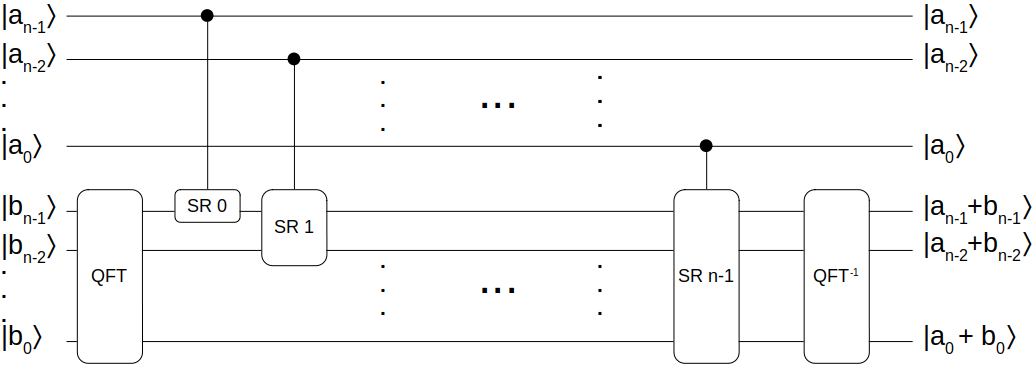
\includegraphics[width=1\textwidth]{qft-adder.png}
  \footnotesize
  \Qcircuit @C=0.35em @R=0.55em {
     & \qw & \gate{\texttt{SR}\;0} & \multigate{3}{\texttt{SR}\;1} & \qw & \qw & \qw & \multigate{5}{\texttt{SR}\;(n-1)} & \qw  \\
      & & & & & \dots & & &  \\
      & \qw & \qw  &  \ghost{\texttt{SR}\; 1} & \qw & \qw & \qw & \ghost{\texttt{SR}\;(n-1)} & \qw \\
      & & & & & & & &  \\
     & & & & & & & &  \\
   & \qw & \qw & \qw & \qw & \qw & \qw & \ghost{\texttt{SR}\;(n-1)}  & \qw 
    }
\end{minipage}
&  
\begin{minipage}{0.25\textwidth}
  \footnotesize
  \Qcircuit @C=0.25em @R=0.35em {
    & \qw & \multigate{3}{(x-a)_n} & \qw \\
    & \vdots & & \\
    & & & \\
    & \qw & \ghost{(x+a)_n} & \qw \\
    }
  \end{minipage}
&
\begin{minipage}{.45\textwidth}
% 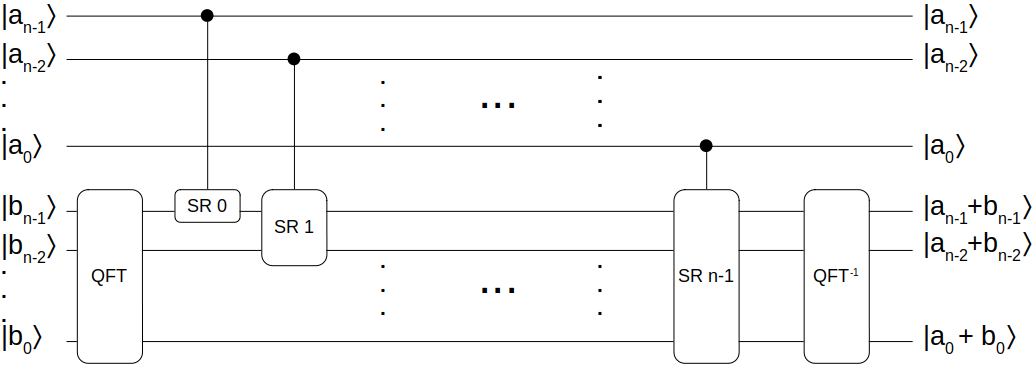
\includegraphics[width=1\textwidth]{qft-adder.png}
  \footnotesize
  \Qcircuit @C=0.35em @R=0.55em {
    & \qw & \multigate{5}{\texttt{SR}^{-1} (n-1)} & \qw & \qw & \qw & \multigate{3}{\texttt{SR}^{-1} 1} & \gate{\texttt{SR}^{-1} 0} & \qw \\
    &     &                                  &     & \dots &   &                              &                      &   \\
    & \qw & \ghost{\texttt{SR}^{-1} (n-1)}        & \qw & \qw   & \qw & \ghost{\texttt{SR}^{-1} 1} & \qw & \qw  \\
      & & & & & & & &  \\
     & & & & & & & &  \\
    & \qw & \ghost{\texttt{SR}^{-1} (n-1)} & \qw & \qw & \qw & \qw & \qw & \qw 
    }
\end{minipage}
\end{tabular}
\caption{Addition/subtraction circuits are inverses}
\label{fig:circuit-add-sub}
\end{figure}

\oqasm programs are easily invertible, as shown by the rules in \Cref{fig:exp-reversed-fun}.
This inversion operation is useful for constructing quantum oracles; for example, the core logic in the QFT-based subtraction circuit is just the inverse of the core logic in the addition circuit (\Cref{fig:exp-reversed-fun}).
This allows us to reuse the proof of addition in the proof of subtraction.
The inversion function satisfies the following properties:

 \begin{theorem}\label{thm:reversibility}\rm[Type reversibility]
    For any well-typed program $\instr$, such that $\Sigma; \Omega \vdash \instr \triangleright \Omega'$, its inverse $\instr'$, where $\instr \xrightarrow{\text{inv}} \instr'$, is also well-typed and we have $\Sigma;\Omega' \vdash \instr' \triangleright \Omega$. Moreover, $\llbracket \instr ; \instr' \rrbracket \varphi=\varphi$.
 \end{theorem}



\section{The full definitions of \qafny}
\label{sec:qafny-app}


\subsection{\qafny Session Generation}

\begin{figure}[t]
{\Small
  \begin{mathpar}
    \inferrule[ ]{ }{\Omega \vdash x : \Omega(x)}

    \inferrule[ ]{\Omega(x)=(x,0,\Sigma(x)) }{\Omega \vdash x[n] : [(x,n,n+1)]}

    \inferrule[ ]{ \Omega \vdash a_1 : q_1 \\ \Omega \vdash a_2 : q_2 }{\Omega \vdash a_1 + a_2 : q_1 \sqcup q_2}   

    \inferrule[ ]{ \Omega \vdash a_1 : q_1 \\ \Omega \vdash a_2 : q_2 }{\Omega \vdash a_1 * a_2 : q_1 \sqcup q_2}   
 

    \inferrule[ ]{ \Omega \vdash a_1 : q_1 \\ \Omega \vdash a_2 : q_2 \Omega \vdash a_3 : q_3  }{\Omega \vdash (a_1 = a_2)@x[n] : q_1 \sqcup q_2\sqcup q_3}   

    \inferrule[ ]{ \Omega \vdash a_1 : q_1 \\ \Omega \vdash a_2 : q_2 \Omega \vdash a_3 : q_3  }{\Omega \vdash (a_1 < a_2)@x[n] : q_1 \sqcup q_2\sqcup q_3}

    \inferrule[ ]{ \Omega \vdash b : q}{\Omega \vdash \neg b : q}  

    \inferrule[ ]{ \Omega \vdash e : \zeta_2 \sqcup \zeta_1 }{\Omega \vdash e : \zeta_1 \sqcup \zeta_2}   

  \end{mathpar}
}
{\footnotesize
\[
\begin{array}{l}
\zeta_1 \sqcup \zeta_2 = \zeta_1 \uplus \zeta_2
\zeta \sqcup g = \zeta
\qquad 
g \sqcup \zeta = \zeta
\qquad
\cmode \sqcup \cmode = \cmode
\qquad
\qmode \sqcup \cmode = \qmode
\qquad
\cmode \sqcup \qmode = \qmode
\qquad
\cmode \le \qmode \le \zeta
\\[0.2em]
\bot \uplus l = l
\qquad 
l \uplus \bot = l

\qquad

[(x,v_1,v_2)] \uplus [(y,v_3,v_4)] = [(x,v_1,v_2), (y,v_3,v_4)]

\\

[v_2,v_2] \cap [v_3,v_4] \neq \emptyset \Rightarrow [(x,v_1,v_2)] \uplus [(x,v_3,v_4)] = [(x,\texttt{min}(v_1,v_3),\texttt{max}(v_2,v_4))]

\end{array}
\]
}
  \caption{Arith, Bool, Gate Mode Checking}
  \label{fig:exp-well-typed}
\end{figure}


A type is written as $\ttype{n}{t}$, where $n$ refers to the total number of qubits in a session,
and $t$ describes the qubit state form. 
A session being type $\ttype{n}{\tnor{\overline{d}}}$
means that every qubit is in normal basis (either $\ket{0}$ or $\ket{1}$),
and $\overline{d}$ describes basis states for the qubits.
The type corresponds to a single qubit basis state $\alpha(n)\ket{\overline{d}}$,
where the global phase $\alpha(n)$ has the form $e^{2 \pi i \frac{1}{n}}$ and $\overline{d}$ is a list of bit values.
Global phases for \texttt{Nor} type are usually ignored in many semantic definitions.
In QWhile, we record it because in quantum conditionals, such global phases might be turned to local phases.

$\ttype{n}{\thad{w}}$ means that every qubit in the session has the state: $(\alpha_1\ket{0} + \alpha_2\ket{1})$;
the qubits are in superposition but they are not entangled.
$\bigcirc$ represents the state is a uniform superposition,
while $\infty$ means the phase amplitude for each qubit is unknown.
If a session has such type, it then has the value form $\Motimes_{k=0}^{m}\ket{\Phi(n_k)}$,
where $\ket{\Phi(n_k)}=\frac{1}{\sqrt{2}}(\ket{0}+\alpha(n_k)\ket{1})$.

All qubits in a session that has type $\ttype{n}{\tch{m}{\beta}}$ are supposedly entangled (eventual entanglement below).
$m$ refers to the number of possible different entangled states in the session,
and the bitstring indexed set $\beta$ describes each of these states, while every element in $\beta$ is indexed by $i\in [0,m)$.
$\beta$ can also be $\infty$ meaning that the entanglement structure is unknown.
For example, in quantum phase estimation, after applying the $\texttt{QFT}^{-1}$ operation, the state has type $\ttype{n}{\tch{m}{\infty}}$. In such case, the only quantum operation to apply is a measurement.
If a session has type $\ttype{n}{\tch{m}{\beta}}$ and the entanglement is a uniform superposition,
we can describe its state as $\sum_{i=0}^{m}{\frac{1}{\sqrt{m}}\beta(i)}$, and the length of bitstring $\beta(i)$ is $n$.
For example, in a $n$-length GHZ application, the final state is: $\ket{0}^{\otimes n}+\ket{1}^{\otimes n}$. 
Thus, its type is $\ttype{n}{\tch{2}{\{\overline{0}^n,\overline{1}^n\}}}$, where $\overline{d}^n$ is a $n$-bit string having bit $d$.

The type $\ttype{n}{\tch{m}{\beta}}$ corresponds to the value form $\sum_{k=0}^{m}\theta_k\ket{\overline{d_k}}$.
$\theta_k$ is an amplitude real number, and $\overline{d_k}$ is the basis.
Basically, $\sum_{k=0}^{m}\theta_k\ket{\overline{d_k}}$ represents a size $m$ array of basis states
that are pairs of $\theta_k$ and $\overline{d_k}$. For a session $\zeta$ of type $\texttt{CH}$,
one can use $\zeta[i]$ to access the $i$-th basis state in the above summation, and the length is $m$.
In the Q-Dafny implementation section, we show how we can represent $\theta_k$ for effective automatic theorem proving.

The QWhile type system has the type judgment: $\Omega,\itau\vdash_g s : \zeta\triangleright \tau$, where $g$ is the context mode, mode environment $\Omega$ maps variables to modes or sessions ($q$ in \Cref{fig:vqimp}), type environment $\itau$ maps a session to its type, $s$ is the statement being typed, $\zeta$ is the session of $s$, and $\tau$ is $\zeta$'s type. 
The QWhile type system in \Cref{fig:exp-sessiontype} has several tasks. First, it enforces context mode restrictions.
Context mode $g$ is either \cmode or \qmode.
$Q$ represents the current expression lives inside a quantum conditional or loop, while \cmode refers to other cases.
In a $Q$ context, one cannot perform $M$-mode operations, i.e., no measurement is allowed.
There are other well-formedness enforcement. For example,
the session of the Boolean guard $b$ in a conditional/loop is disjoint with the session in the conditional/loop body,
i.e., qubits used in a Boolean guard cannot appear in its conditional/loop body.

Second, the type system enforces mode checking for variables and expressions in \Cref{fig:exp-well-typed}.
In QWhile, \cmode-mode variables are evaluated to values during type checking.
In a \texttt{let} statement (\Cref{fig:exp-sessiontype}),
\cmode-mode expression is evaluated to a value $n$, and the variable $x$ is replaced by $n$ in $s$.
The expression mode checking (\Cref{fig:exp-well-typed}) has the judgment: $\Omega \vdash (a\mid b) : q$. It takes a mode environment $\Omega$, and an expression ($a$, $b$), and judges if the expression has the mode $g$ if it contains only classical values, or a quantum session $\zeta$ if it contains some quantum values. 
All the supposedly \cmode-mode locations in an expression are assumed
to be evaluated to values in the type checking step,
such as the index value $x[n]$ in difference expressions in \Cref{fig:exp-well-typed}.
It is worth noting that the session computation ($\uplus$)
is also commutative as the last rule in \Cref{fig:exp-well-typed}.

Third, by generating the session of an expression, the QWhile type system assigns a type $\tau$ for the session indicating its state format, which will be discussed shortly below. Recall that a session is a list of quantum qubit fragments.
In quantum computation, qubits can entangled with each other.
We utilize type $\tau$ (\Cref{fig:vqir-state}) to state entanglement properties appearing in a group of qubits.
It is worth noting that the entanglement property refers to \textit{eventual entanglement}, .i.e. a group of qubits that are eventually entangled. Entanglement classification is tough and might not be necessary. In most near term quantum algorithms, such as Shor's algorithm \cite{shors} and Childs' Boolean equation algorithm (BEA) \cite{ChildsNAND}, programmers care about if qubits eventually become entangled during a quantum loop execution. This is why the normal basis type ($\ttype{n}{\tnor{\overline{d}}}$) can also be a subtype of a entanglement type ($\ttype{n}{\tch{1}{\{\overline{d}\}}}$) in our system (\Cref{fig:exp-subtyping}).

\myparagraph{Entanglement Types}
We first investigate the relationship between the types and entanglement states.
It is well-known that every single quantum gate application
does not create entanglement ($\texttt{X}$, $\texttt{H}$, and $\texttt{RZ}$).
It is enough to classify entanglement effects through a control gate application, i.e., 
$\sifq{x[i]}{e(y)}$, where the control node is $x[i]$ and $e$ is an operation applying on $y$.

A qubit can be described as $\alpha_1\ket{b_1}+\alpha_2\ket{b_2}$,
where $\alpha_1$/$\alpha_2$ are phase amplitudes, and $b_1$/$b_2$ are bases.
For simplicity, we assume that
when we applying a quantum operation on a qubit array $y$, we either solely change the qubit amplitudes or bases.
We identify the former one as $\mathpzc{R}$ kind, referring to its similarity of applying an \texttt{RZ} gate;
and the latter as $\mathpzc{X}$ kind, referring to its similarity of applying an \texttt{X} gate.
The entanglement situation between $x[i]$ and $y$ after applying a control statement $\sifq{x[i]}{e(y)}$ is described in \Cref{fig:control-entanglement}.

\begin{figure*}[t]
{\footnotesize
\begin{tabular}{|c|c|c|c|c|c|c|c|c|c|}
\hline                           
&  Case 1 & Case 2 & Case 3 & Case 4 & Case 5 & Case 6 & Case 7 & Case 8 & Case 9 \\
\hline
$x[i]$ & \texttt{Nor} & \texttt{Had} & \texttt{Had} & \texttt{Had} & \texttt{Had} & \texttt{Had} & \texttt{Had} & \texttt{CH} & \texttt{CH} \\
$y$  & any & \texttt{Nor} & \texttt{Nor} & \texttt{Had} & \texttt{Had} & \texttt{CH} & \texttt{CH} & \texttt{CH} & \texttt{CH}   \\\hline
$y$'s operation type  & any & $\mathpzc{X}$ & $\mathpzc{R}$ & $\mathpzc{X}$ & $\mathpzc{R}$ & $\mathpzc{X}$ & $\mathpzc{R}$ &  $\mathpzc{X}$ & $\mathpzc{R}$ \\\hline
Output Type Entangled?  & N & Y & N & N & Y & Y & Y & Y & Y  \\
\hline                           
\end{tabular}
  \caption{Control Gate Entanglement Situation}
  \label{fig:control-entanglement}
}
\end{figure*}

If $x[i]$ has input type \texttt{Nor}, the control operation acts as a classical conditional, i.e., no entanglement is possible.
In most quantum algorithms, $x[i]$ will be in superposition (type \texttt{Had}) to enable entanglement creation.
When $y$ has type $\texttt{Nor}$, if $y$'s operation is of $\mathpzc{X}$ kind, an entanglement between $x[i]$ and $y$ is created, such as the GHZ algorithm; 
if the operation is of $\mathpzc{R}$ kind, there is not entanglement after the control application, such as the Quantum Phase Estimation (QPE) algorithm.

When $x[i]$ and $y$ are both of type \texttt{Had}, if we apply an $\mathpzc{X}$ kind operation on $y$,
it does not create entanglement. An example application is the phase kickback pattern.
If we apply a $\mathpzc{R}$ operation on $y$, this does create entanglement.
This kind of operations appears in state preparations, such as preparing a register $x$ to have state $\sum_{t=0}^N i^{-t}\ket{t}$ in Childs' Boolean equation algorithm \cite{ChildsNAND}. 
The main goal for preparing such state is not to entanglement qubits, but to prepare a state with phases related to its bases.

\begin{figure}[t]
{\small
$
\begin{array}{l}
\ttype{n}{\tnor{\overline{d}}} \sqsubseteq \ttype{n}{\tch{1}{\{\overline{d}\}}}
\qquad 
\ttype{n}{\tch{2^n}{\beta}} \sqsubseteq \ttype{n}{\tch{2^n}{\infty}}
\qquad 
\ttype{n}{\thad{\bigcirc}} \sqsubseteq \ttype{n}{\tch{2^n}{\tpower{n}}}
\end{array}
$
}
  \caption{Session Type Subtyping}
  \label{fig:exp-subtyping}
\end{figure}

The case when $x[i]$ and $y$ has type \texttt{Had} and \texttt{CH}, respectively,
happens in the middle of executing a quantum loop, such as in the Shor's algorithm and BEA.
Applying both $\mathpzc{X}$ and $\mathpzc{R}$ kind operations result in entanglement.
In this narrative, algorithm designers intend to
merge an additional qubit $x[i]$ into an existing entanglement session $y$.
$x[i]$ is commonly in uniform superposition,
but there can be some additional local phases attached with some bases,
which we named this situation as saturation, i.e.,
In an entanglement session written as $\sum_{i=0}^n \ket{x_l,y,x_r}$,
for any fixing $x_l$ and $x_r$ bases, if $y$ covers all possible bases,
we then say that the part $y$ in the entanglement is in saturation.
This concept is important for generating auto-proof, which will be discussed in \Cref{sec:logical}.


When $x[i]$ and $y$ are both of type \texttt{CH}, there are two situations.
When the two parties belong to the same entanglement session,
it is possible that an $\mathpzc{X}$ or $\mathpzc{R}$ operation de-entangles the session.
Since QWhile tracks eventual entanglement.
In many cases, \texttt{HAD} type can be viewed as a kind of entanglement.
In addition, the QWhile type system make sure that most de-entanglements happen
at the end of the algorithm by turning the qubit type to $\tch{m}{\infty}$,
so that after the possible de-entanglement, the only possible application is a measurement.

If $x[i]$ and $y$ are in different entanglement sessions,
the situation is similar to when $x[i]$ having \texttt{Had} and $y$ having \texttt{CH} type.
It merges the two sessions together through the saturation $x[i]$.
For example, in BEA, The quantum Boolean guard computes the following operation $(z < i) @ x[i]$
on a \texttt{Had} type variable $z$ (state: $\sum_{k=0}^{2^n}\ket{k}$)
and a $\texttt{Nor}$ type factor $x[i]$ (state: $\ket{0}$).
The result is an entanglement $\sum_{k=0}^{2^n}\ket{k,k < i}$,
where the $x[i]$ position stores the Boolean bit result $k < i$. \footnote{When $k<i$, $x[i]=1$ while $\neg (k<i)$, $x[i]=0$.}
The algorithm further merges the $\ket{z,x[i]}$ session with a loop body entanglement session $y$. 
In this cases, both $\ket{z,x[i]}$ and $y$ are of \texttt{CH} type. 

